\documentclass{article}

% packages
\usepackage{amsmath, amsthm, thmtools, amsfonts, amssymb, luacode, catchfile, tikzducks, hyperref, ifthen}
\ifcsname c@kobocompile\endcsname
	\usepackage[a5paper, total={1072pt, 1448pt}, margin=10pt, includeheadfoot]{geometry} % set page margins
\else
	\usepackage[a4paper, margin=50pt, includeheadfoot]{geometry}
\fi
\usepackage[shortlabels]{enumitem}
\usepackage[skip=3pt, indent=0pt]{parskip}

% language
\usepackage[bidi=basic, layout=tabular, provide=*]{babel}
\ifcsname c@english\endcsname
	\babelprovide[main, import]{english}
\else
	\babelprovide[main, import]{hebrew}
	\babelprovide{rl}
\fi
%\babelfont{rm}{Libertinus Serif}
\babelfont{rm}[Renderer=Harfbuzz]{Libertinus Serif}
\babelfont{sf}{Libertinus Sans}
\babelfont{tt}{Libertinus Mono}

% style
\AddToHook{cmd/section/before}{\clearpage}	% Add line break before section
\linespread{1.3}
\setcounter{secnumdepth}{0}		% Remove default number tags from sections, this won't do well with theorems
\AtBeginDocument{\setlength{\belowdisplayskip}{3pt}}
\AtBeginDocument{\setlength{\abovedisplayskip}{3pt}}
\graphicspath{ {../images/} }

% operators
\DeclareMathOperator\cis{cis}
\DeclareMathOperator\Sp{Sp}
\DeclareMathOperator\tr{tr}
\DeclareMathOperator\im{Im}
\DeclareMathOperator\re{Re}
\DeclareMathOperator\diag{diag}
\DeclareMathOperator*\lowlim{\underline{lim}}
\DeclareMathOperator*\uplim{\overline{lim}}
\DeclareMathOperator\rng{rng}
\DeclareMathOperator\Sym{Sym}
\DeclareMathOperator\Arg{Arg}
\DeclareMathOperator\Log{Log}
\DeclareMathOperator\dom{dom}
\DeclareMathOperator\supp{Supp}
\DeclareMathOperator\var{Var}
\DeclareMathOperator\cov{Cov}

% commands
%\renewcommand\qedsymbol{\textbf{מש''ל}}
%\renewcommand\qedsymbol{\fbox{\emoji{lizard}}}
\newcommand{\Aa}[0]{\mathcal{A}}
\newcommand{\Bb}[0]{\mathcal{B}}
\newcommand{\CC}[0]{\mathbb{C}}
\newcommand{\Cc}[0]{\mathcal{C}}
\newcommand{\EE}[0]{\mathbb{E}}
\newcommand{\FF}[0]{\mathbb{F}}
\newcommand{\Ff}[0]{\mathcal{F}}
\newcommand{\Ii}[0]{\mathcal{I}}
\newcommand{\Gg}[0]{\mathcal{G}}
\newcommand{\Ll}[0]{\mathcal{L}}
\newcommand{\Mm}[0]{\mathcal{M}}
\newcommand{\NN}[0]{\mathbb{N}}
\newcommand{\Nn}[0]{\mathcal{N}}
\newcommand{\PP}[0]{\mathbb{P}}
\newcommand{\Pp}[0]{\mathcal{P}}
\newcommand{\QQ}[0]{\mathbb{Q}}
\newcommand{\RR}[0]{\mathbb{R}}
\newcommand{\Rr}[0]{\mathcal{R}}
\newcommand{\Ss}[0]{\mathcal{S}}
\newcommand{\TT}[0]{\mathbb{T}}
\newcommand{\Uu}[0]{\mathcal{U}}
\newcommand{\Vv}[0]{\mathcal{V}}
\newcommand{\Ww}[0]{\mathcal{W}}
\newcommand{\ZZ}[0]{\mathbb{Z}}
\newcommand{\acts}[0]{\circlearrowright}
\newcommand{\explain}[2] {
	\begin{flalign*}
		 && \text{#2} && \text{#1}
	\end{flalign*}
}
\newcommand{\maketitleprint}[0]{ \begin{center}
	%\begin{tikzpicture}[scale=3]
	%	\duck[graduate=gray!20!black, tassel=red!70!black]
	%\end{tikzpicture}	
	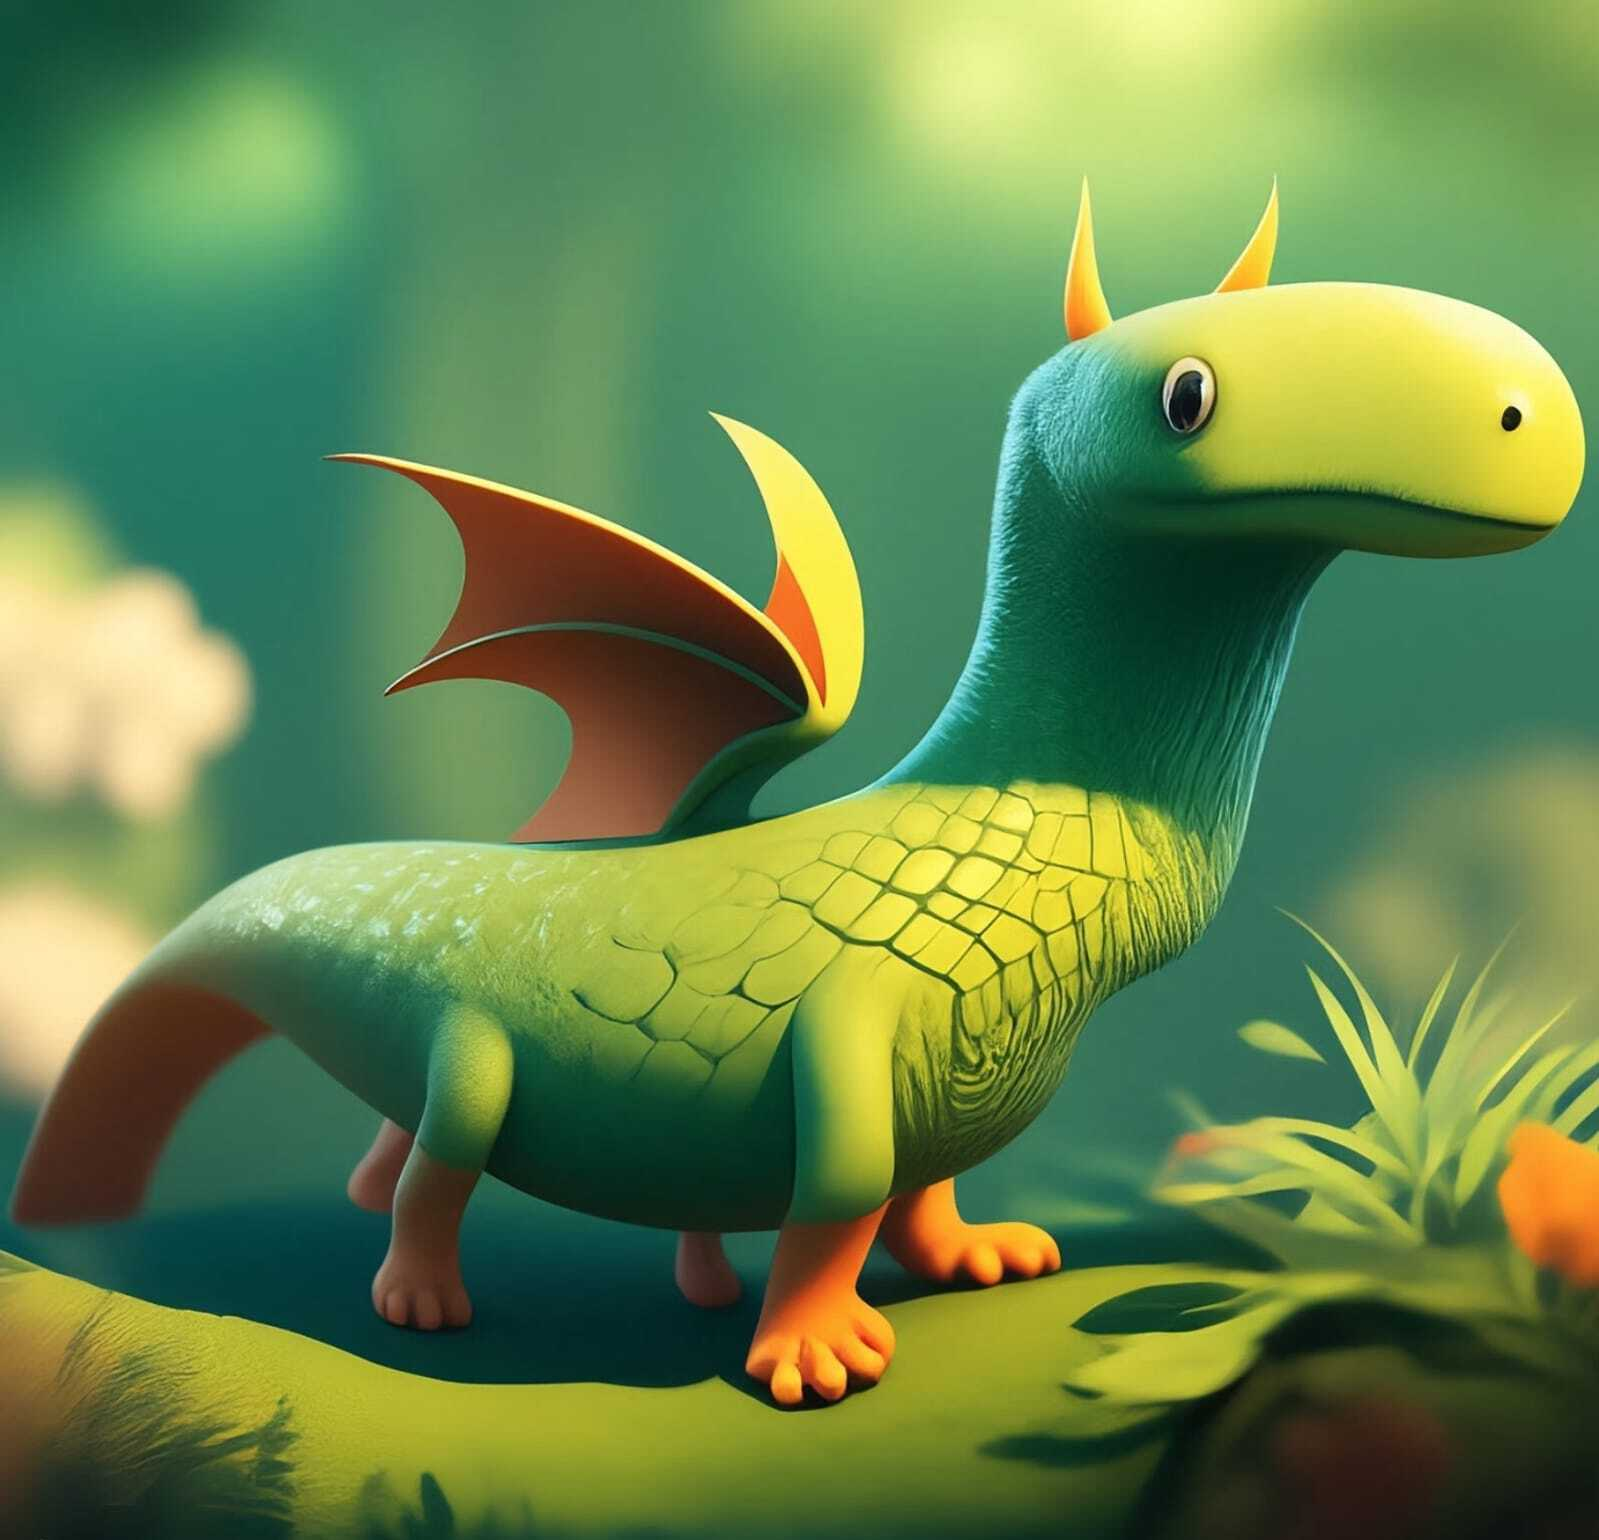
\includegraphics[width=6cm]{cover}
\end{center}
}

% theorem commands
\newtheoremstyle{c_remark}
	{}	% Space above
	{}	% Space below
	{}% Body font
	{}	% Indent amount
	{\bfseries}	% Theorem head font
	{}	% Punctuation after theorem head
	{.5em}	% Space after theorem head
	{\thmname{#1}\thmnumber{ #2}\thmnote{ \normalfont{\text{(#3)}}}}	% head content
\newtheoremstyle{c_definition}
	{3pt}	% Space above
	{3pt}	% Space below
	{}% Body font
	{}	% Indent amount
	{\bfseries}	% Theorem head font
	{}	% Punctuation after theorem head
	{.5em}	% Space after theorem head
	{\thmname{#1}\thmnumber{ #2}\thmnote{ \normalfont{\text{(#3)}}}}	% head content
\newtheoremstyle{c_plain}
	{3pt}	% Space above
	{3pt}	% Space below
	{\itshape}% Body font
	{}	% Indent amount
	{\bfseries}	% Theorem head font
	{}	% Punctuation after theorem head
	{.5em}	% Space after theorem head
	{\thmname{#1}\thmnumber{ #2}\thmnote{ \text{(#3)}}}	% head content

\ifcsname c@english\endcsname
	\theoremstyle{plain}
	\newtheorem{theorem}{Theorem}[section]
	\newtheorem{lemma}[theorem]{Lemma}
	\newtheorem{proposition}[theorem]{Proposition}
	\newtheorem*{proposition*}{Proposition}
	%\newtheorem{corollary}[theorem]{אין חלופה עברית}

	\theoremstyle{definition}
	\newtheorem{definition}[theorem]{Definition}
	\newtheorem*{definition*}{Definition}
	\newtheorem{example}{Example}[section]
	\newtheorem{exercise}{Exercise}[section]

	\theoremstyle{remark}
	\newtheorem*{remark}{Remark}
	\newtheorem*{solution}{Solution}
	\newtheorem{conclusion}[theorem]{Conclusion}
	\newtheorem{notation}[theorem]{Notation}
\else
	\theoremstyle{c_plain}
	\newtheorem{theorem}{משפט}[section]
	\newtheorem{lemma}[theorem]{למה}
	\newtheorem{proposition}[theorem]{טענה}
	\newtheorem*{proposition*}{טענה}
	%\newtheorem{corollary}[theorem]{אין חלופה עברית}

	\theoremstyle{c_definition}
	\newtheorem{definition}[theorem]{הגדרה}
	\newtheorem*{definition*}{הגדרה}
	\newtheorem{example}{דוגמה}[section]
	\newtheorem{exercise}{תרגיל}[section]

	\theoremstyle{c_remark}
	\newtheorem*{remark}{הערה}
	\newtheorem*{solution}{פתרון}
	\newtheorem{conclusion}[theorem]{מסקנה}
	\newtheorem{notation}[theorem]{סימון}
\fi

% Questions related commands
\newcounter{question}
\setcounter{question}{1}
\newcounter{sub_question}
\setcounter{sub_question}{1}

\ifcsname c@english\endcsname
	\newcommand{\question}[1][0]{
		\ifthenelse{#1 = 0}{}{\setcounter{question}{#1}}
		\section{Question \arabic{question}}
		\addtocounter{question}{1}
		\setcounter{sub_question}{1}
	}

	\newcommand{\subquestion}[1][0]{
		\ifthenelse{#1 = 0}{}{\setcounter{sub_question}{#1}}
		\subsection{Part \alph{sub_question}}
		\addtocounter{sub_question}{1}
	}
\else
	\newcommand{\question}[1][0]{
		\ifthenelse{#1 = 0}{}{\setcounter{question}{#1}}
		\section{שאלה \arabic{question}}
		\addtocounter{question}{1}
		\setcounter{sub_question}{1}
	}

	\newcommand{\subquestion}[1][0]{
		\ifthenelse{#1 = 0}{}{\setcounter{sub_question}{#1}}
		\subsection{סעיף \localecounter{letters.gershayim}{sub_question}}
		\addtocounter{sub_question}{1}
	}
\fi

% import lua and start of document
\directlua{common = require ('../common')}

\GetEnv{AUTHOR}

% headers
\author{\AUTHOR}
\date\today

\title{פתרון מטלה 02 --- מבוא ללוגיקה, 80423}

\begin{document}
\maketitle
\maketitleprint{}

\Question{}
תהי שפה $L = \{P, Q, R, S\}$ ויהי $\varphi = (\lnot ((P \to (\lnot Q)) \land ((\lnot R) \lor S)))$. \\*
נכתוב עץ בינארי סטנדרטי מיושר לשמאל $(T, f)$ ל־$\varphi$, ונחשב את הפונקציה המתאימה $\psi$.
\begin{solution}
	נגדיר
	\begin{align*}
		f = \{
			& (\langle \rangle, \lnot),
			(\langle 0, 0, 1 \rangle, \lnot),
			(\langle 0, 1, 0 \rangle, \lnot),
			(\langle 0 \rangle, \land),
			(\langle 0, 0 \rangle, \rightarrow), \\
			& (\langle 0, 1 \rangle, \lor),
			(\langle 0, 0, 0 \rangle, P),
			(\langle 0, 0, 1, 0 \rangle, Q),
			(\langle 0, 1, 0, 0 \rangle, R),
			(\langle 0, 1, 1 \rangle, S)
		\}
	\end{align*}
	עוד נגדיר $T = (\text{dom} f, \preceq)$ כאשר $\preceq$ יחס הרישא חד־מקומי, ובהתאם $(T, f)$ עץ היצירה של $\varphi$.

	נגדיר $\psi : T \to \text{sent}_L$, נקבל
	\begin{align*}
		\psi = \{
			& ( \langle \rangle, (\lnot ((P \to (\lnot Q)) \land ((\lnot R) \lor S))) ), \\
			& ( \langle 0 \rangle, ((P \to (\lnot Q)) \land ((\lnot R) \lor S)) ), \\
			& ( \langle 0, 0 \rangle, (P \to (\lnot Q)) ), \\
			& ( \langle 0, 0, 0 \rangle, P ), \\
			& ( \langle 0, 0, 1 \rangle, (\lnot Q) ), \\
			& ( \langle 0, 0, 1, 0 \rangle, Q ), \\
			& ( \langle 0, 1 \rangle, ((\lnot R) \lor S) ), \\
			& ( \langle 0, 1, 0 \rangle, (\lnot R) ), \\
			& ( \langle 0, 1, 0, 0 \rangle, R ), \\
			& ( \langle 0, 1, 1 \rangle, S )
		\}
	\end{align*}
\end{solution}

\Question{}
תהי $L$ שפה, נוכיח שהביטוי $p \in \exp_L$ הוא פסוק אם ורק אם הוא פסוק מוגדר קווית.
\begin{proof}
	נוכיח ש־$sent_L^+$ תת־קבוצה מינימלית של $\exp_L$ הסגורה תחת $F_\lnot, F_\square$ לכל $\square \in B$. \\*
	נניח כי $\varphi \in sent_L^+$ ונגדיר $S \subseteq \exp_L$ הקבוצה המינימלית עליה דיברנו, עוד נניח כי $\varphi \notin L$, דהינו הקבוצה $sent_L^+$ לא מינימלית בגללה. \\*
	מהגדרת $sent_L^+$ קיימת סדרת יצירה ל־$\varphi$, נגדירה כ־$(\varphi_0, \dots, \varphi_n = \varphi)$.
	עתה נוכיח באינדוקציה על אורך הרשימה כי $\varphi \in S$. כבסיס נניח שאורך הרשימה 1, לכן $\varphi_0 = \varphi \in S$ וסיימנו.
	נניח עתה כי אורך הרשימה הוא $n$, ועוד נניח כי לכל $0 \le k < n$ מתקיים $\varphi_k \in S$, נוכיח כי גם $\varphi_n \in S$.
	אילו $\varphi_n \in L$ אז סיימנו, אילו מתקיים $\varphi_n = (\lnot \varphi_k)$ עבור $0 \le k < n$ אז נקבל ש־$\varphi_n = F_\lnot(\varphi_k)$ אבל $\varphi_k \in S$ ולכן גם $F_\lnot(\varphi_k)$ ולכן גם $\varphi \in S$.
	נניח אם כן שמתקיים $\varphi = (\varphi_i \square \varphi_j)$ עבור $0 \le i, j < n$, נקבל אם כן $\varphi_i, \varphi_j \in S$, ובהתאם $F_\square(\varphi_i, \varphi_j) \in S$, וקיבלנו כי בכל מקרה $\varphi \in S$.
	השלמנו את צעד האינדוקציה ולכן קיבלנו שמתקיים $sent_L^+ \subseteq S \subseteq sent_L^+$ ולכן $S = sent_L^+$ בלבד.

	נוכיח עתה גם כי $sent_L \subseteq S$, נגדיר $\varphi$ מחדש על־ידי $\varphi \in sent_L$, לכן ל־$\varphi$ עץ יצירה $(T, f)$.
	נוכיח באינדוקציה על גובה העץ כי $\varphi \in S$, כבסיס נניח כי גובה העץ 1, לכן אין עוקבים ל־$\langle \rangle$, אז נובע כי $\varphi \in L$ ולכן גם $\varphi \in S$.
	נניח כי הטענה נכונה עבור גובה עץ $0 \le k < n$ ונניח כי גובה $T$ הוא $n$. לא יתכן כי ל־$\langle \rangle$ אין עוקבים, לכן או שיש לו עוקב או שיש לו שניים.
	אילו יש לו עוקב יחיד, אז מתקיים $\varphi = (\lnot \psi_{\langle 0 \rangle})$, כאשר ל־$\psi_{\langle 0 \rangle}$ עץ יצירה באורך $n - 1$, לכן הוא מוכל ב־$S$ ובהתאם $\varphi \in S$.
	נניח אם כן שיש שני עוקבים ל־$\langle \rangle$, נסמנם $\psi_0, \psi_1$, ונקבל כי אורך עץ היצירה של שניהם $n - 1$ ולכן גם $\psi_0, \psi_1 \in S$.
	נקבל כי גם $F_{f(\langle \rangle)}(\psi_0, \psi_1) \in S$, אבל $F_{f(\langle \rangle)}(\psi_1, \psi_2) = \varphi$, לכן $\varphi \in S$ והשלמנו את מהלך האינדוקציה.
	נסיק אם כן $S \subseteq sent_L \subseteq S$ ולכן בהכרח $S = sent_L$.

	נסיק $sent_L = S = sent_L^+$, דהינו $sent_L = sent_L^+$.
\end{proof}

\Question{}
תהי $L$ שפה לתחשיב פסוקים, $X$ קבוצה, $h : L \to X$ פונקציה, $\epsilon_\lnot : X \to X$ פונקציה ו־$\epsilon_\square : X^2 \to X$ פונקציה לכל $\square \in B$.

\directlua{ C_number = 2 }
\Subquestion{}
נוכיח כי קיימת פונקציה $\bar{h} : sent_L \to X$ כך ש־$\forall \varphi \in L, \bar{h}(\varphi) = h(\varphi)$ וכן $\forall \varphi = (\lnot \psi), \bar{h}(\varphi) = \epsilon_\lnot(\bar{h}(\psi))$
ועבור כל $\square \in B$ מתקיים $\varphi = (\psi_0 \square \psi_1) \implies \bar{h}(\varphi) = \epsilon_\square(\bar{h}(\psi_0), \bar{h}(\psi_1))$.
\begin{proof}
	יהי $\psi \in sent_L$, לכן קיים עץ יצירה $(T_\psi, f_\psi)$ עבורו. \\*
	ניזכר בשאלה 3 ממטלה 1 ונגדיר את $\tilde{g}_{\psi, (T_\psi, f_\psi)} : T_\psi \to X$ הפונקציה היחידה המקיימת לכל עלה בעץ היצירה $\tilde{g}_{\psi, (T_\psi, f_\psi)}(t) = h(f(t))$,
	לכל $t \in T_\psi$ בעל עוקב יחיד $\tilde{g}_{\psi, (T_\psi, f_\psi)}(t) = \epsilon_\lnot(\tilde{g}_{\psi, (T_\psi, f_\psi)}(t \frown \langle 0 \rangle))$
	וכן לכל $t \in T_\psi$ בעל שני עוקבים $\tilde{g}_{\psi, (T_\psi, f_\psi)}(t) = \epsilon_{f(t)}(\tilde{g}_{\psi, (T_\psi, f_\psi)}(t \frown \langle 0 \rangle), \tilde{g}_{\psi, (T_\psi, f_\psi)}(t \frown \langle 1 \rangle))$. \\*
	נגדיר עתה $\bar{h}(\psi) = \tilde{g}_{\psi, (T_\psi, f_\psi)}(\langle \rangle)$ ונבדוק שהתנאים אכן מתקיימים. \\*
	תחילה נבחין כי ממסקנה מהכיתה נובע כי עץ היצירה לכל פסוק הוא יחיד, לכן הגדרה זו יחד עם יחידות $g$ היא תקפה, ונוכל לדון לא בתוקפה אלא בקיום התכונות הרצויות בלבד. \\*
	נניח כי $\psi \in L^1$, אז מתקיים $\bar{h}(\psi) = \tilde{g}_{\psi, (T_\psi, f_\psi)}(\langle \rangle) = h(f_\psi(\langle \rangle)) = h(\psi)$. \\*
	עתה נשתמש בטענה זו כבסיס למהלך אינדוקטיבי על מבנה הפסוק, נניח כי הטענה נכונה עבור $\varphi$ ועוד נניח שמתקיים $\psi = (\lnot \varphi)$,
	אז נקבל $\bar{h}(\psi) = \tilde{g}_{\psi, (T_\psi, f_\psi)}(\langle \rangle) = \epsilon_\lnot(\tilde{g}_{\psi, (T_\psi, f_\psi)}(\langle 0 \rangle)) = \epsilon_\lnot(\bar{h}(\varphi))$,
	נבחין כי השתמשנו פה פעמיים בהגדרה שסיפקנו ל־$\bar{h}$.
	נניח אם כן שמתקיים $\psi = (\varphi_0 \square \varphi_1)$ עבור $\square \in B$,
	ואז $\bar{h}(\psi) = \tilde{g}_{\psi, (T_\psi, f_\psi)}(\langle \rangle) = \epsilon_{f_\psi(\langle \rangle)}(\tilde{g}_{\psi, (T_\psi, f_\psi)}(\langle 0 \rangle), \tilde{g}_{\psi, (T_\psi, f_\psi)}(\langle 1 \rangle))
	= \epsilon_\square(\bar{h}(\varphi_0), \bar{h}(\varphi_1))$, ושוב קיבלנו כי התכונה של $\bar{h}$ נשמרת, והשלמנו את המהלך האינדוקטיבי. \\*
	בהתאם נוכל להסיק כי $\bar{h}$ לא רק מוגדרת באופן חזק, אלא גם מקיימת את שלושת התנאים.
\end{proof}

\Subquestion{}
נוכיח כי הפונקציה $\bar{h}$ מוגדרת ביחידות.
\begin{proof}
	תהינה $\bar{h}, \bar{h}'$ שתי פונקציות המקיימות את התנאים. \\*
	יהי $\psi \in L$, מהתכונות שמצאנו מתקיים $\bar{h}(\psi) = h(\psi)$ אך גם $\bar{h}'(\psi) = h(\psi)$ ולכן בפרט $\bar{h}(\psi) = \bar{h}'(\psi)$. \\*
	גם הפעם נשתמש בטענה זו כבסיס האינדוקציה על מבנה הפסוק, ולכן נניח עתה את מהלך האינדוקציה, דהינו יהי $\varphi \in sent_L$ כך ש־$\bar{h}(\varphi) = \bar{h}'(\varphi)$, ויהי $\psi = (\lnot \varphi)$.
	לכן $\bar{h}(\psi) = \epsilon_\lnot(\bar{h}(\varphi)) = \epsilon_\lnot(\bar{h}'(\varphi)) = \bar{h}'(\psi)$ ושוב הגענו לשוויון. \\*
	נניח אם כך $\varphi_0, \varphi_1 \in sent_L$ מקיימים את הטענה, ונגדיר $\psi = (\varphi_0 \square \varphi_1)$ עבור $\square \in B$. \\*
	אז $\bar{h}(\psi) = \epsilon_\square(\bar{h}(\varphi_0), \bar{h}(\varphi_1)) = \epsilon_\square(\bar{h}'(\varphi_0), \bar{h}'(\varphi_1)) = \bar{h}'(\psi)$. \\*
	השלמנו אם כך את מהלך האינדוקציה וקיבלנו ש־$\bar{h}$ היא אכן יחידה.
\end{proof}

\Question{}
תהי $L$ שפה לתחשיב פסוקים.

\Subquestion{}
נוכיח כי אם $\varphi \in sent_L$ אז יש לו אינסוף סדרות יצירה שונות.
\begin{proof}
	תהי $\alpha_0 = \langle \varphi_0, \dots, \varphi_{n - 1} \rangle$ סדרת יצירה כך ש־$\varphi = \varphi_0$. \\*
	נניח כי $\psi \in L$ פסוק יסודי כלשהו שמובטחל שקיים מהגדרת $L$. \\*
	עתה נבנה סדרה חדשה $\alpha_1 = \langle \varphi \rangle \frown \alpha_0$.
	נבחין כי כל תנאי סדרת היצירה נשמרו שכן האיבר הראשון לא מצריך איברים נוספים, ולכל איבר כל האיברים הקודמים לו נשמרו ברשימה ובסדר. \\*
	ביתר פירוט נוכל להוכיח באינדוקציה על אורך הרשימה כי אכן $\alpha_1$ סדרת יצירה של $\varphi$. \\*
	עתה נבצע תהליך זה באופן מחזורי, נגדיר $\alpha_k = \langle \psi \rangle \frown \alpha_{k - 1}$.
	כמובן אורך $\alpha_k$ שונה לכל $k \in \NN$ ולכן הסדרות אכן שונות.
\end{proof}

\Subquestion{}
עתה נגדיר $L = \{ p, q \}$, ונחשב את מספר סדרות היצירה השונות של הפסוק $\varphi = (p \to q)$ כך שהן באורך 3.
\begin{solution}
	נגדיר $\langle \varphi_0, \varphi_1, \varphi_2 \rangle$ סדרת יצירה של $\varphi$, לכן גם $\varphi_2 = \varphi$. \\*
	מהגדרת סדרת יצירה קיים $0 \le i \le 2$ כך ש־$p$ מופיע בסדרה וכך גם עבור $q$, זאת מטענה $\varphi = \varphi_2$, נבחין כי מצב זה יתכן כאשר $\varphi_0 = p, \varphi_1 = q$ או כאשר $\varphi_0 = q, \varphi_1 = p$ בלבד.
	נסיק אם כן שמספר הסדרות באורך 3 הוא 2 בלבד.
\end{solution}

\end{document}
